Una vez definidos los requisitos del cliente y con la información expuesta en la sección \ref{sec:DocRequisitos} podemos comenzar a idear el funcionamiento de nuestra página web.

En la siguiente sección vamos a modelar el funcionamiento de nuestra web en diversas áreas. En primer lugar presentamos varios modelos IFML (\textit{Interaction Flow Modeling Language})\cite{IFML:Design} en los que se representa el flujo de comportamiento de nuestra aplicación web. A continuación usaremos UML (\textit{Unified Modeling Language})\cite{UMLWebsite} para mostrar las relaciones entre las diferentes entidades presentes en la aplicación y cómo se comunican entre ellas. Por último, vemos un diagrama de despliegue en el que vemos como se realiza el lanzamiento de la aplicación para poder ser usada por el usuario.

\subsection{Modelo en IFML}

Para realizar el modelo IFML de nuestra aplicación, que pretende definir el comportamiento de la misma en función de las acciones del usuario, nos hemos basado en los requisitos descritos en la sección \ref{sec:DocRequisitos}. Esto es así para intentar cumplir al máximo de nuestras posibilidades las expectativas del cliente.

\begin{figure}
	\centering
	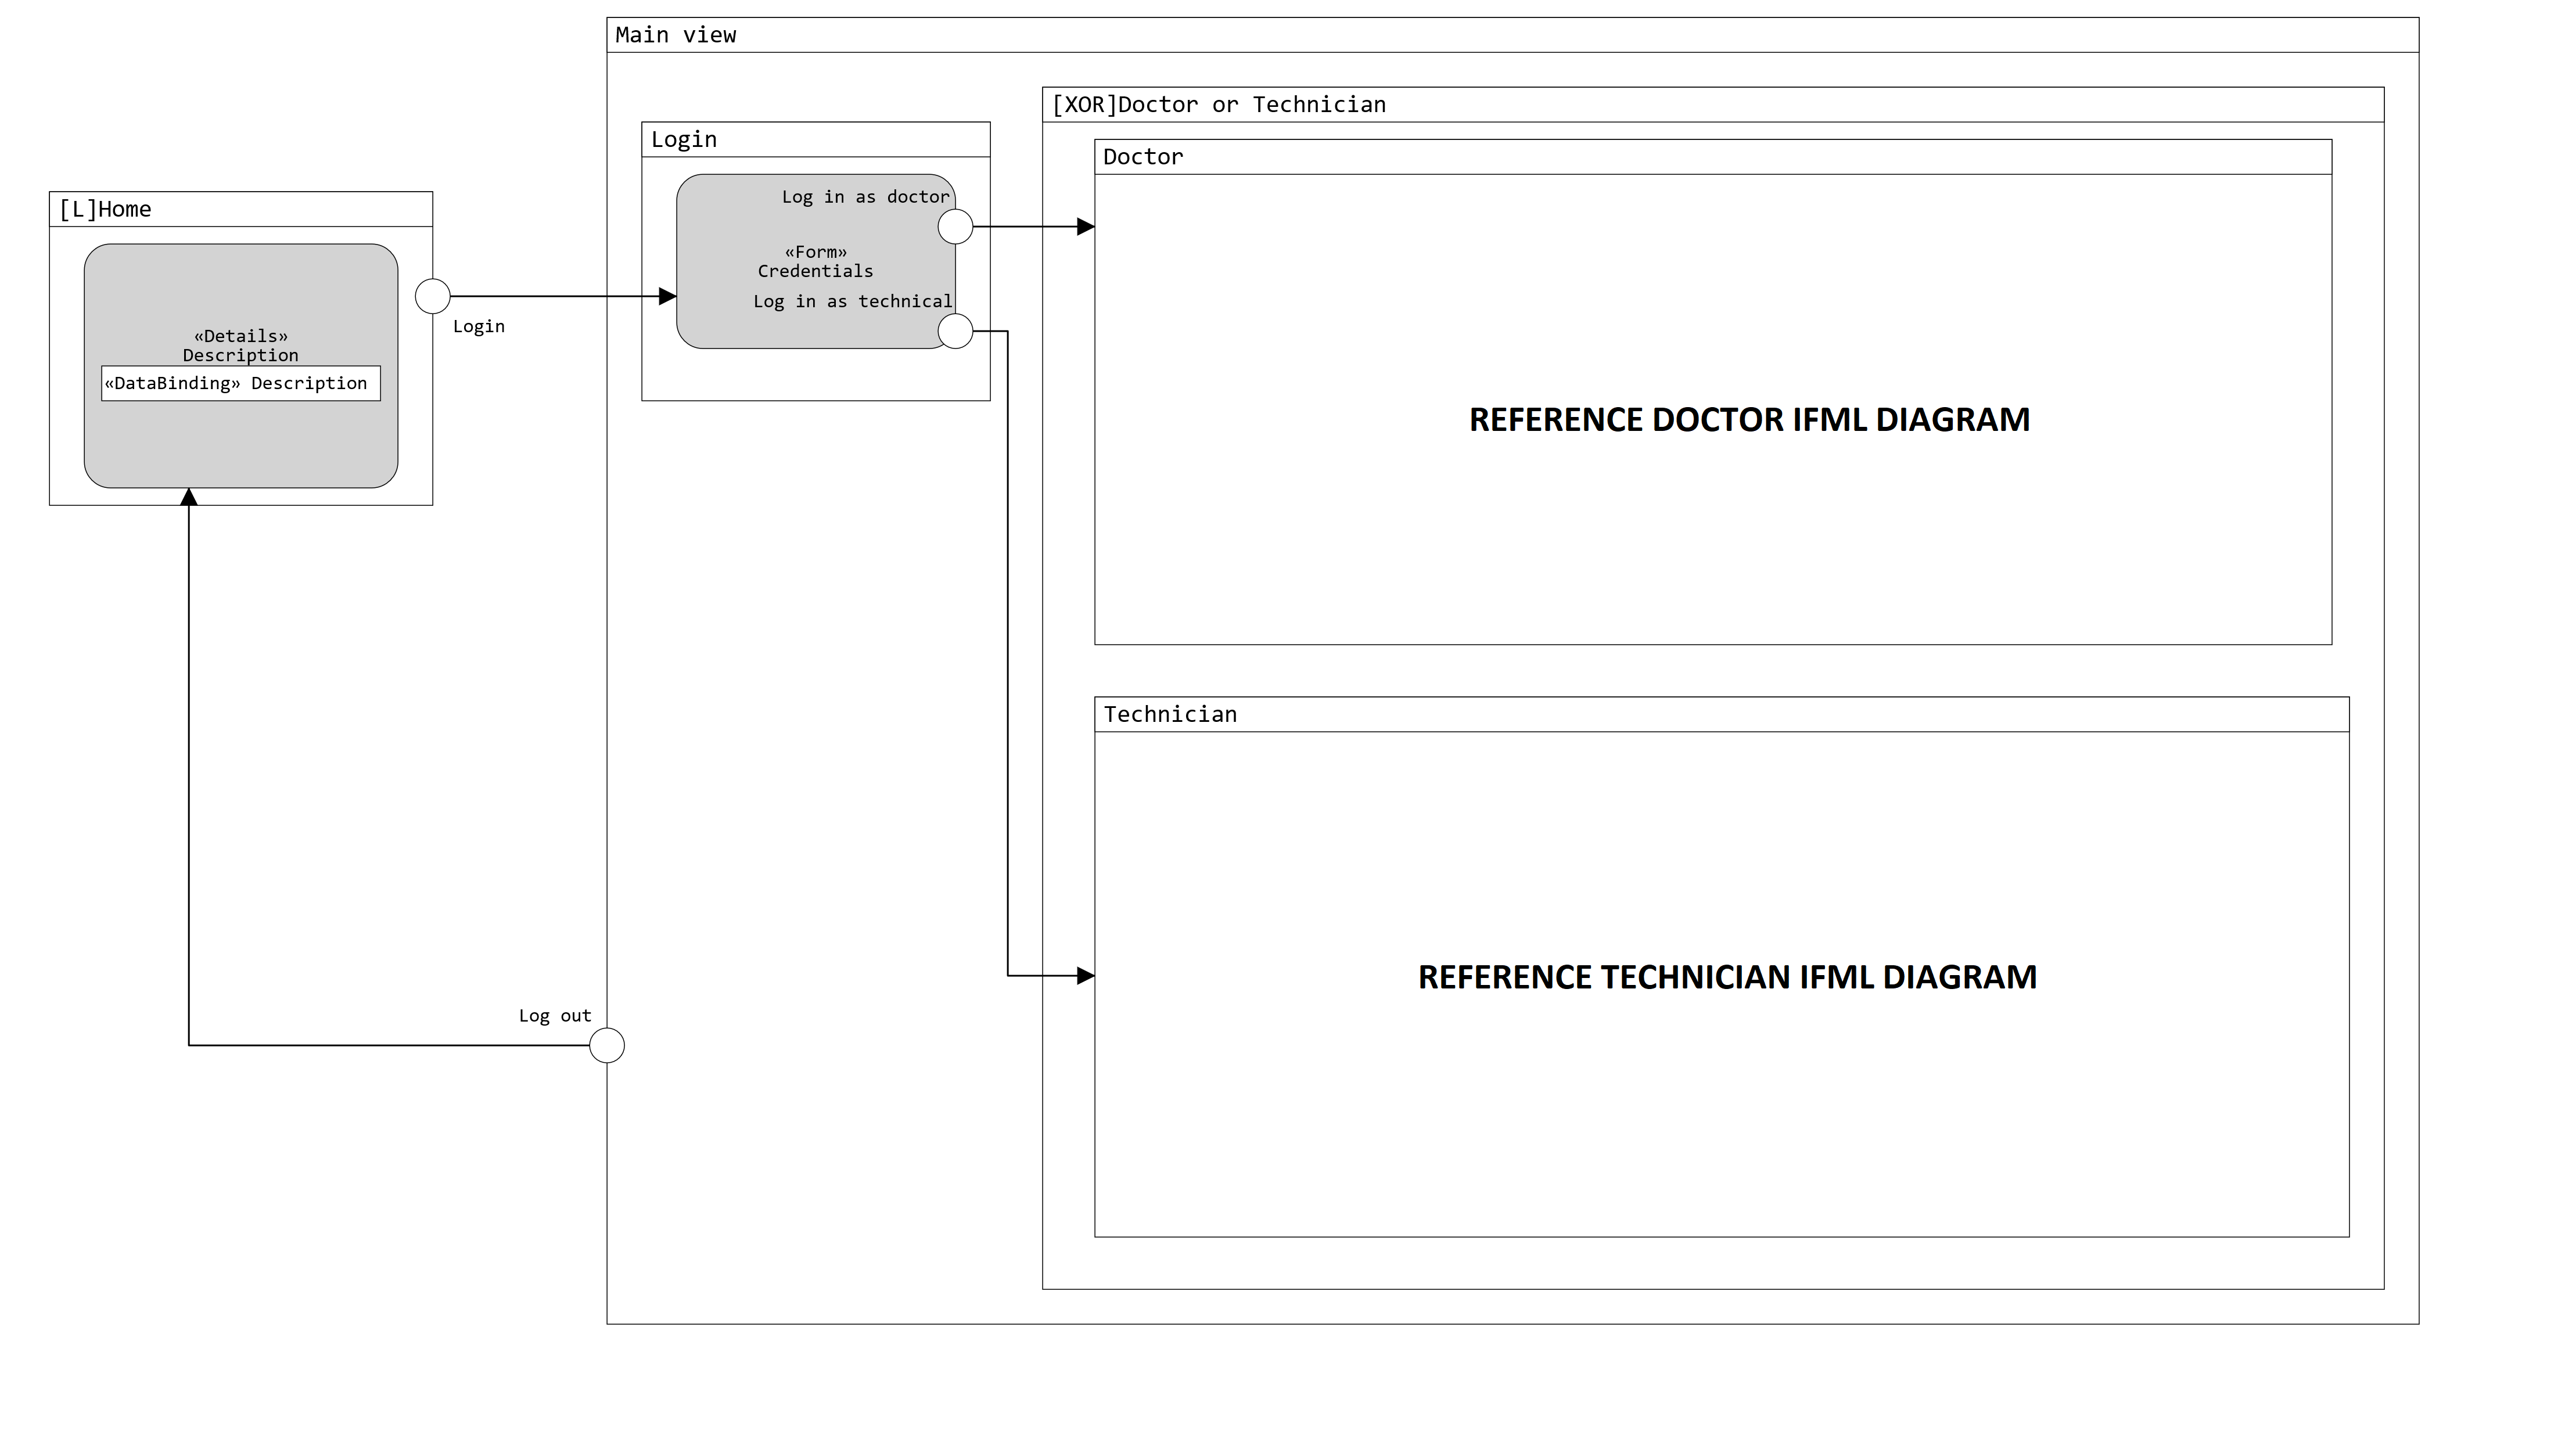
\includegraphics[width=\textwidth]{images/General-IFML.png}
	\caption{Modelo IFML general de la aplicación. Véase las figuras \ref{fig:IFMLDoctor} y \ref{fig:IFMLTech} para completar la información}
	\label{fig:IFMLModel}
\end{figure}

\begin{figure}
	\centering
	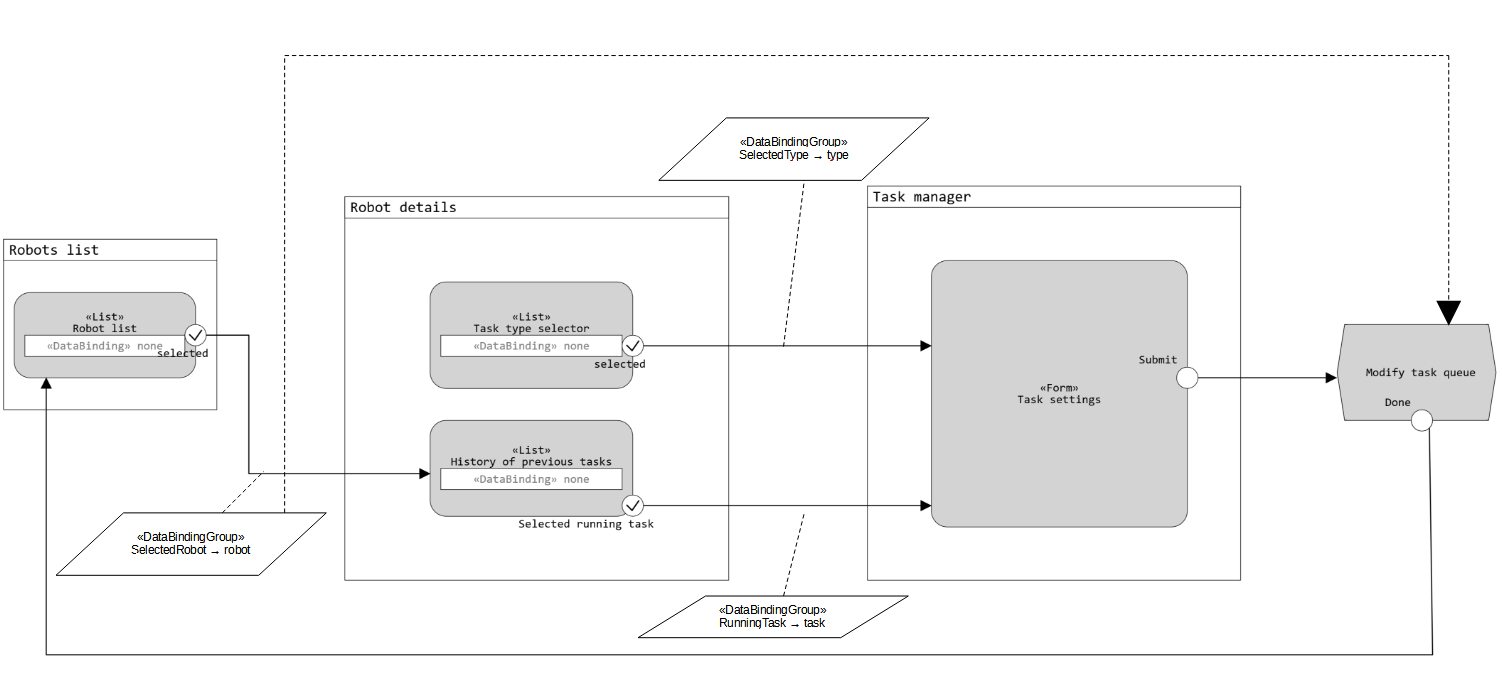
\includegraphics[width=1\textwidth]{images/Doctor-IFML.PNG}
	\caption{Modelo IFML concreto de la vista del médico}
	\label{fig:IFMLDoctor}
\end{figure}

\begin{figure}
	\centering
	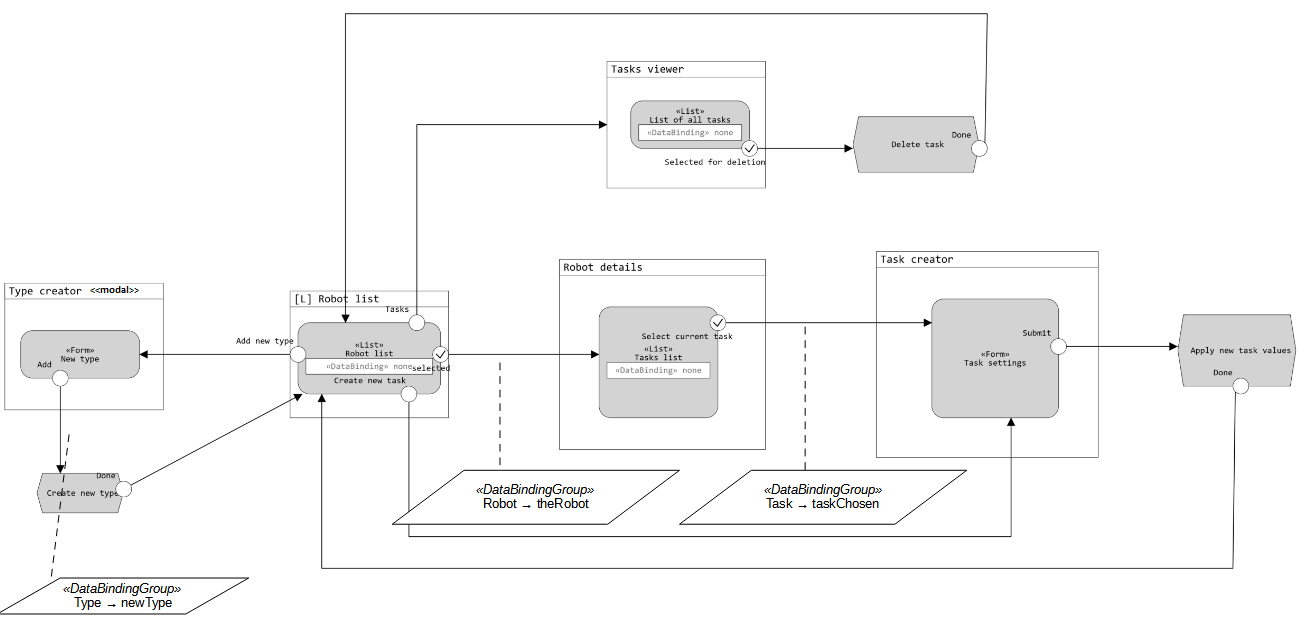
\includegraphics[width=1\textwidth]{images/Tech-IFML.PNG}
	\caption{Modelo IFML concreto de la vista del técnico}
	\label{fig:IFMLTech}
\end{figure}

Como podemos observar en la figura \ref{fig:IFMLModel}, la web dispondrá de una pantalla de inicio, con la posibilidad de iniciar sesión, lo que representa el requisito F-10.

Dentro del contenedor \textit{Main View}, tendremos diferentes \textit{View Containers} dependiendo si el usuario es un empleado sanitario o bien, un técnico.

Si el usuario es un personal sanitario, usará el contenedor \textit{Doctor}. En él, el usuario podrá visualizar una lista con todos los robots y sus respectivos estados (ocupado, libre o error). Dicha característica implementa los requisitos funcionales RF-4, RF-7 y RF-12. 

Además, el usuario podrá seleccionar un robot en concreto de dicha lista, lo cual desplegará la información completa de ese robot (su tarea actual, problemas surgidos y el historial de tareas de la última jornada), y también permitirá asignar una nueva tarea o bien cancelarla. Dichas características reflejan los requisitos funcionales RF-1, RF-2, RF-3, RF-4, RF-7, RF-8, RF-9 Y RF-11.

Todas las acciones de gestión de tareas descritas anteriormente se actualizarán en el robot afectado con la acción \textit{Modify task queue} y se volverá a la lista de robots anterior.

Si el usuario es un técnico, obtendremos un comportamiento similar al anterior. En este caso, el contenedor a usar será \textit{Technician}. En él, el usuario podrá visualizar una lista con todos los tipos de robots existentes. Dicha característica implementa el requisito RF-5. Si el técnico elige un determinado tipo, se mostrará un formulario con todas las posibles tareas que dicho tipo de robot puede ejecutar. Además, permitirá modificar, eliminar y añadir tareas. Dichas características representan los requisitos funcionales RF-6 y RF-9.

Todas las acciones de gestión descritas anteriormente se actualizarán en los robots del mismo tipo con la acción \textit{Update tasks for robot} y se volverá a la lista de tipos de tarea anterior.

\subsection{Diseño de lógica}

\begin{figure}[H]
	\centering
	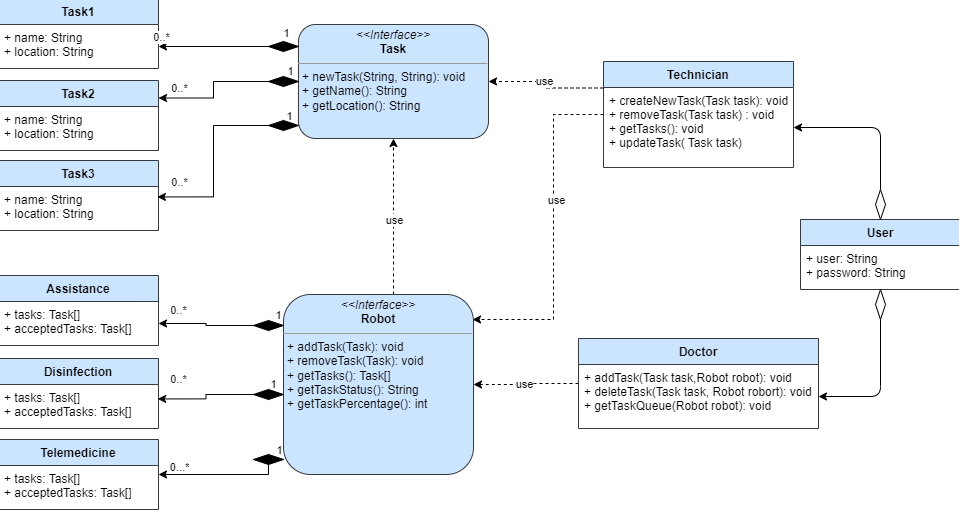
\includegraphics[width=1\textwidth]{images/class-diagram.png}
	\caption{UML class diagram}
	\label{fig:UMLModel}
\end{figure}
 Tal y como podemos ver en la Figura \ref{fig:UMLModel}, el sistema estará formado por la clase \textit{User}, la cual guardará el usuario y contraseña. Esta clase tiene dos hijos: \textit{Technician} y \textit{Doctor}.
 
 La clase \textit{Technician} se relaciona con la interfaz de tareas \textit{Task}, mediante relaciones de uso para crear, eliminar o modificar el funcionamiento de las tareas, y con la interfaz \textit{Robot}, para poder crear nuevos tipos de robots. \textit{Doctor} también tiene una relación de uso con la interfaz \textit{Robot} para poder añadir o eliminar tareas de la cola de tareas correspondiente al robot que se quiera modificar. La interfaz \textit{Robot} será implementada, en principio, por tres tipos de robots: \textit{Assistance}, \textit{Disifection} y \textit{Telemedicine}. Sin embargo el modelo permite crear facilmente nuevos tipos de robots con diferentes funcionalidades y nos ofrece mayor escalabilidad. Esto es así también para las tareas, ya que la interfaz\textit{Task} nos permite crear gran cantidad de tareas interoperables sin problema. Como podemos observar, se cumplen casi por completo los requisitos funcionales requeridos por el usuario, lo que hace indicarnos que con este diagrama estamos eligiendo el camino correcto en nuestro desarrollo del proyecto. 
 
Las acciones mostradas en el IFML se realizarán de la siguiente forma desde las clases:

\begin{itemize}
  \item \textbf{Modify task queue}. Para ello, se usará la clase Doctor en la que se pasarán como parámetros el robot seleccionado y se realizarán las tareas seleccionadas por el usuario, es decir, si el empleado sanitario añade una tarea a un robot, se usará el método \textit{addTask}, para eliminar una tarea asignada se usará el método \textit{deleteTask} y para consultar la información de un robot, se usará el método \textit{getTaskOfRobot}.
  
  \item \textbf{Apply new tasks values}. Para ello, se usará la clase Technician. Si el técnico desea crear un nuevo tipo de tarea, se usará el método \textit{createNewTask}, para eliminar tipo de tareas, se usará el método \textit{removeTask} y para poder visualizar todos los tipos de tarea para un robot en concreto, se usará el método \textit{getAllTaskTypes}. Finalmente, si el técnico desea actualizar el funcionamiento de alguna tarea en concreto de un robot, usará el método \textit{updateTaskType}.
\end{itemize}

\subsection{Diagrama de despliegue}

Por último, en la figura \ref{fig:deploy} podemos observar el diagrama de despliegue que tendrá nuestra web. Al ser de uso local en los hospitales en los que vaya a utilizarse no necesitaremos del uso de bases de datos podremos guardar toda la información necesaria en el disco local de la máquina servidor. Esto ayudará a la web a ser mucho más rápida y eficiente ya que una web estática necesita de menos recursos para su funcionamiento y además no sufre de bajas latencias cuando se produzcan caídas de conexión. Por otro lado podemos observar que se utilizará HTML para utilizar la web, lenguaje que todos los navegadores conocen y pueden mostrarlo al usuario. Por último el servidor web alojará una aplicación de flask que será la encargada de realizar todos los procesos necesarios para el funcionamiento de la web.

\begin{figure}[H]
	\centering
	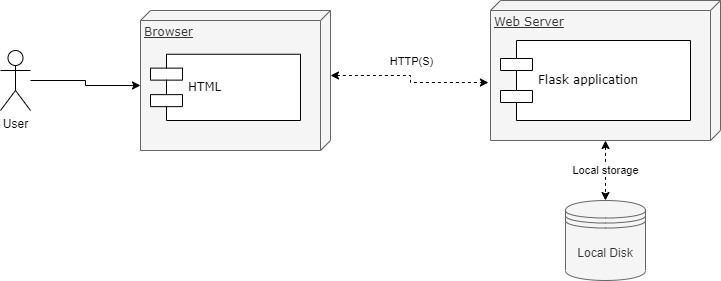
\includegraphics[width=1\textwidth]{images/diagramaDespliegueWeb.png}
	\caption{Diagrama de despliegue}
	\label{fig:deploy}
\end{figure}


\newpage